\documentclass{minimal}
\usepackage{graphicx,color}
\usepackage[utf8]{inputenc}
\usepackage[papersize={335.00bp,251.00bp},text={335.00bp,251.00bp}]{geometry}
\begin{document}
\centering
% Title: Figure 2
% Creator: GL2PS 1.4.2, (C) 1999-2020 C. Geuzaine
% For: Octave
% CreationDate: Tue Dec 13 23:14:40 2022
\setlength{\unitlength}{1pt}
\begin{picture}(0,0)
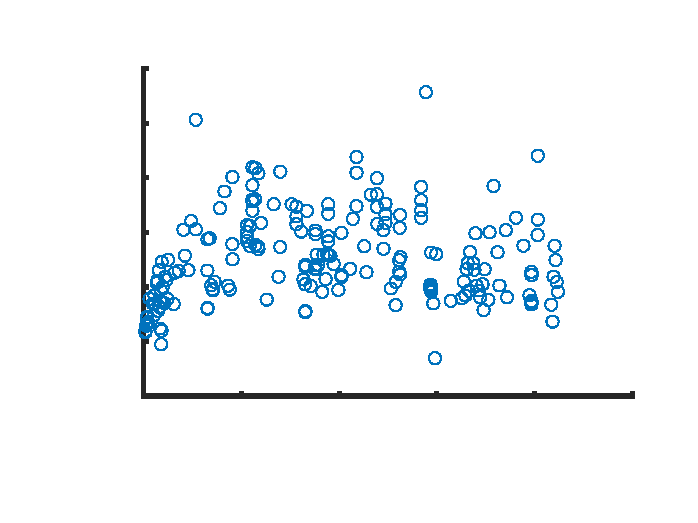
\includegraphics[scale=1]{DoubleKapitzaPoincare-inc}
\end{picture}%
\begin{picture}(335,251)(0,0)
\fontsize{22}{0}\selectfont\put(68.978,44.4581){\makebox(0,0)[t]{\textcolor[rgb]{0.15,0.15,0.15}{{0}}}}
\fontsize{22}{0}\selectfont\put(115.889,44.4581){\makebox(0,0)[t]{\textcolor[rgb]{0.15,0.15,0.15}{{200}}}}
\fontsize{22}{0}\selectfont\put(162.799,44.4581){\makebox(0,0)[t]{\textcolor[rgb]{0.15,0.15,0.15}{{400}}}}
\fontsize{22}{0}\selectfont\put(209.71,44.4581){\makebox(0,0)[t]{\textcolor[rgb]{0.15,0.15,0.15}{{600}}}}
\fontsize{22}{0}\selectfont\put(256.62,44.4581){\makebox(0,0)[t]{\textcolor[rgb]{0.15,0.15,0.15}{{800}}}}
\fontsize{22}{0}\selectfont\put(303.531,44.4581){\makebox(0,0)[t]{\textcolor[rgb]{0.15,0.15,0.15}{{1000}}}}
\fontsize{22}{0}\selectfont\put(57.9989,60.9621){\makebox(0,0)[r]{\textcolor[rgb]{0.15,0.15,0.15}{{-10}}}}
\fontsize{22}{0}\selectfont\put(57.9989,87.1351){\makebox(0,0)[r]{\textcolor[rgb]{0.15,0.15,0.15}{{0}}}}
\fontsize{22}{0}\selectfont\put(57.9989,113.308){\makebox(0,0)[r]{\textcolor[rgb]{0.15,0.15,0.15}{{10}}}}
\fontsize{22}{0}\selectfont\put(57.9989,139.481){\makebox(0,0)[r]{\textcolor[rgb]{0.15,0.15,0.15}{{20}}}}
\fontsize{22}{0}\selectfont\put(57.9989,165.654){\makebox(0,0)[r]{\textcolor[rgb]{0.15,0.15,0.15}{{30}}}}
\fontsize{22}{0}\selectfont\put(57.9989,191.827){\makebox(0,0)[r]{\textcolor[rgb]{0.15,0.15,0.15}{{40}}}}
\fontsize{22}{0}\selectfont\put(57.9989,218){\makebox(0,0)[r]{\textcolor[rgb]{0.15,0.15,0.15}{{50}}}}
\fontsize{24}{0}\selectfont\put(186.255,24.4581){\makebox(0,0)[t]{\textcolor[rgb]{0.15,0.15,0.15}{{$\theta_2/(2 \pi)$}}}}
\fontsize{24}{0}\selectfont\put(23.9989,139.481){\rotatebox{90}{\makebox(0,0)[b]{\textcolor[rgb]{0.15,0.15,0.15}{{$\omega_2$}}}}}
\fontsize{24}{0}\selectfont\put(186.255,228){\makebox(0,0)[b]{\textcolor[rgb]{0,0,0}{{Poincaré Section at $\theta_1 = 0$}}}}
\end{picture}
\end{document}
